%!TEX root = ../thesis.tex
%*******************************************************************************
%*********************************** Introduction Chapter *****************************
%*******************************************************************************

\chapter{Introduction}
\graphicspath{{Chapter_Intro/Figs/}}

The pursuit of three-dimensional (3D) displays has continued at a pace over the past 20 years. Currently, most commercially-available `3D display' products such as 3D cinema, 3D TV, handheld 3D devices (e.g. Nintendo 3DS, HTC Evo 3D) and Virtual Reality (VR) and Augmented Reality (AR) head sets are in fact stereoscopic displays \cite{McIntire2014} where two different two-dimensional (2D) images are displayed to the left and right eyes respectively, creating a 3D illusion in the brain. Despite their high image quality, the major issue with stereoscopic displays is that they cannot provide real optical defocusing effect in depth \cite{Watt2005}. Modern 3D cinemas are able to provide good comfort because polarisation glasses are as light as regular glasses, and the variable defocusing issue can be avoided by the combinations of good design of point of interest in each scene and the according defocusing effect as captured by the camera, so most audience won't experience much discomfort for around 2 to 3 hours, which has contributed to the general acceptance of 3D films by the public \cite{Barbara2013}. However, the content, viewing angle and depth of focus of 3D films are fixed after they are captured. To provide an interactive and real-time rendered immersive experience, VR/AR headsets have frequently been advertised as the `gateway to the metaverse' in recent years \cite{IET_metaverse_report2022}. However, personal experiences with VR headsets are far from comfortable, not only because of their heavy weight, but also because the display is physically at a very close distance. This creates an unnatural experience because the brain perceives objects at various distances while keeping them all in focus, but in real life, when focusing on a near object, the background naturally blurs. Moreover, the two displays in the VR headset need to be rendered in real-time based on the location and viewing angle of the user, so delays in rendering often cause dizziness and sickness. Hence, the heavy weight, the lack of real depth of focus and the delay in rendering collectively cause discomfort, dizziness and sickness to VR headsets users \cite{McCauley1992, Chang2020}.

In comparison, holography techniques can produce a full 3D light field, which does not rely on any head mounted device, has true depth of focus, and does not need to be re-rendered according to change in viewer position and viewing angle.

\begin{figure}[H]
    \centering
    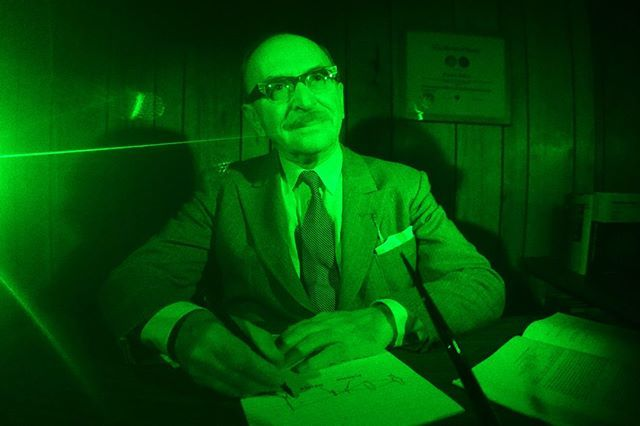
\includegraphics[width=0.6\textwidth]{Dennis-Gabor-Hologram-2.jpg}
    \caption{A photo of the holographic portrait of Dennis Gabor \cite{Lo2018}}\label{fig:Dennis-Gabor-Hologram-2}
\end{figure}

Holography, taking its name from the Greek word $o \lambda o \sigma $ (holos), meaning \textit{whole}, was first introduced in 1948 by Dennis Gabor \cite{Gabor1948}, originally named as \textit{wavefront reconstruction} \cite{Hecht2017}. It is a technology which generates 3D images via the diffraction of light. Similar to 2D photography, the earliest holography used a piece of film to record the diffraction pattern, which was then used to reconstruct the 3D field, as shown in \cref{fig:Dennis-Gabor-Hologram-2} (which is a holographic recording of Dennis Gabor himself). After the invention of digital cameras, digital holography emerged. The limitation of both methods is that they require a physical object prior to recording the hologram. In order to generate hologram for objects that do not physically exist, computer-generated holography (CGH) was developed. In CGH, a hologram can be calculated through various algorithmic approaches and then displayed on a spatial light modulator (SLM) that modulates the wavefront of a coherent light source to produce 3D reconstructions. Currently available SLM's can only modulate either phase or amplitude, so algorithms are needed to compute amplitude-only or phase-only holograms. The classic phase-retrieval algorithms include direct binary search \cite{Seldowitz1987}, simulated annealing \cite{Kirkpatrick1983} and Gerchberg-Saxton \cite{Gerchberg1972}. With the developments in modern numerical optimisation methods and increases in computational power, phase retrieval using numerical optimisation methods has also been found in the literature, such as the gradient descent \cite{Zhang2017, Liu2020} and its stochastic variations \cite{Chen2021, Choi2021, Kadis2022}. However, all the existing phase retrieval methods still have some fundamental issues, primarily related to their poor image quality and/or the heavy computation required, the solutions of which are the ultimate goals of this research.

This thesis therefore explores the development and optimisation of phase-only CGHs for holographic displays. The research investigates various phase retrieval algorithms and proposes novel methods to enhance the reconstruction quality and computational efficiency of CGHs, and then investigates the fundamental limits of discretised phase holograms from an information theory point of view. The thesis is structured as following.

Chapter 2 provides a comprehensive literature review, covering the fundamental theories of light, the principles of holography and the evolution of CGH methods. The chapter reviews various phase retrieval algorithms, including the Direct Binary Search (DBS), Simulated Annealing (SA), Gerchberg-Saxton (GS), One-Step Phase Retrieval (OSPR) and Adaptive One-Step Phase Retrieval (AD-OSPR) algorithms and their adaptations for 3D CGHs, emphasising the limitations of current algorithms and introducing the motivation for pursuing more advanced CGH techniques.

Chapter 3 proposes the Digital Pre-Distorted One-Step Phase Retrieval (DPD-OSPR) method. By experimentally evaluating the non-linearities in the holographic projection system and applying a digital pre-distortion (DPD) curve, this chapter demonstrates significant improvements in reconstruction quality and reductions in mean squared error.

Chapter 4 introduces the optimisation of phase-only holograms using the Limited-memory Broyden-Fletcher-Goldfarb-Shanno (L-BFGS) optimisation algorithm, and then proposes the novel Target Image Phase Optimisation (TIPO) technique, which optimises the phase of the target image instead of the phase of the hologram. Then the multi-depth phase-only hologram optimisation for 3D targets is investigated, and a novel technique called Sequential Slicing (SS) is proposed, which evaluates the loss for a single slice of the 3D target at each iteration instead of a full evaluation on all slices, reducing computational time while maintaining overall quality and minimising quality imbalances across all slices.

Chapter 5 extends the optimisation method on generating time-multiplexing binary-phase holograms and proposes the novel Multi-Frame Holograms Batched Optimisation (MFHBO) technique. By optimising a batch of holograms for time multiplexing, the finite response time of human vision is leveraged to average out noise, resulting in improved visual quality. The MFHBO algorithm demonstrates much better quality compared to the existing time-multiplexing hologram generation methods, such as OSPR and AD-OSPR.

Chapter 6 investigates the information capacity of phase-only CGH. This chapter examines the effects of quantisation on hologram bit depth and their impact on reconstruction quality, and looks for the correlation between the entropy of the target image and the reconstruction error, providing insights into the fundamental limits of discretised CGH.

Chapter 7 marks the conclusion and lists potential further work that could be done.
